\chapter{Proposta de solução}

Neste capítulo serão apresentados os componentes e procedimentos utilizados na elaboração da proposta de solução, denominada ``BURI''. Conforme as
etapas definidas na metodologia, ocorre inicialmente a discussão sobre a fase de pesquisa na Seção \ref{fase1}, seguida pela especificação 
das funcionalidades e comportamento do sistema BURI, contextualizados na Seção \ref{fase2}. O particionamento e execução de atividades nas áreas de 
\textit{hardware} e \textit{software} são explicados nas Seções \ref{fase3} e \ref{fase4}, respectivamente. Na Seção \ref{fase5},  o aplicativo Android e o 
dispositivo físico são avaliados por um grupo selecionado de alunos, a fim de garantir a usabilidade do sistema proposto e, posteriormente, são produzidas a documentação 
do projeto e guia de instalação na Seção \ref{fase6}. 

\section{Pesquisa}\label{fase1}

A primeira fase consiste na compreensão do problema. O objetivo é encontrar trabalhos semelhantes sobre o uso de IoT no monitoramento da qualidade do ar, assim 
como as consequências fisiológicas de inalação prolongada de monóxido de carbono, e identificar, através de um questionário aplicado aos alunos, as preocupações relacionadas 
ao tema no ambiente doméstico.

Em primeiro lugar, realizou-se uma revisão da literatura para identificar pesquisas no âmbito de tecnologias IoT e monitoramento do ar com foco 
em prevenção de acidentes, porém foram selecionados cinco trabalhos acadêmicos para o desenvolvimento da proposta e comparação de funcionalidades. 
Além disso, o estudo da intoxicação por monóxido de carbono visa investigar as consequências para a saúde humana. Portanto, a explicação científica sobre o tema é do 
artigo ``Carbon monoxide poisoning: a review for clinicians'' \cite{carbon-monoxide-poisoning-varon}, pois o conteúdo inclui 
explicação técnica e didática do processo de envenenamento, consequências no sistema neurológico e cardiovascular, fontes de contaminação e métodos de tratamento utilizados na medicina.

Por fim, foi aplicado um questionário a um grupo de estudantes da Escola Superior de Tecnologia da Universidade do Estado do Amazonas (EST/UEA), para coletar informações acerca de suas
preocupações em relação à qualidade do ar no ambiente doméstico. A pesquisa teve como propósito identificar as características do ambiente residencial desses alunos e avaliar seu 
nível de conscientização sobre os riscos associados aos poluentes atmosféricos. Participaram deste levantamento inicial 58 estudantes matriculados em cursos da área de Engenharia, os quais responderam 
ao questionário de forma voluntária.

As respostas do questionário são relevantes para a construção do protótipo. Como destaque, algumas informações importantes serão analisadas a seguir. Segundo a pesquisa, 
75,9\% dos estudantes utilizam um \textit{smartphone} com 
Sistema Operacional Android, pois a tecnologia é fonte de acesso à informação e inclusão digital no Brasil \cite{impacto-android-brasil}. Outro aspecto analisado foi 
a percepção dos alunos em relação à qualidade do ar em suas residências e arredores. Nas respostas, os relatos sobre a presença de fumaça e dificuldade respiratória em dias específicos foram comuns. Como relatou um dos alunos: ``a fumaça se tornou um problema pra resolver isso decidimos comprar um umidificador de ar''. 

Evidência do problema apresentado, a Universidade do Estado do Amazonas (UEA) suspende atividades presenciais nos dias 19 e 20 de setembro na capital e interior por causa 
da alta quantidade de poluentes, pois os índices ultrapassaram a marca de 125 $\mu m/m^{3}$ e um ar de boa qualidade permite a concentração de partículas em  até 25 $\mu m/m^{3}$ \cite{uea-queima-fecha}. Portanto, 
o funcionamento de um dispositivo de medição em tempo real com interface para dispositivo móvel representa uma boa alternativa para auxílio do usuário.

\begin{figure}[ht]
    \centering
    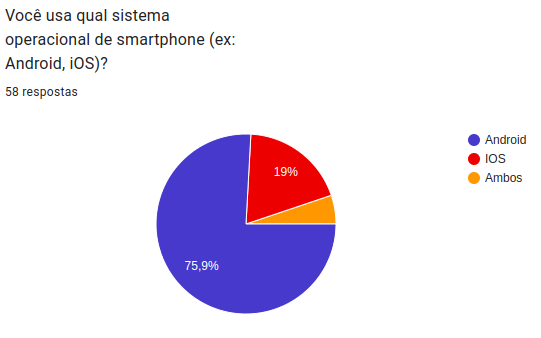
\includegraphics[width=.67\textwidth]{img/graf1-SO-smartphone.png}
    \caption{Sistemas Operacionais dos \textit{smartphones} dos alunos da EST. Fonte:Autor}\label{figSOsmartphone}
\end{figure}

Sobre o tipo de conexão com a internet, a figura \ref{figWifiAlunos} ilustra a porcentagem de estudantes com rede Wi-Fi em suas residências. De acordo com a pesquia,  
a maioria dos entrevistados possui acesso à rede Wi-Fi. Esse valor é especialmente útil para a viabilidade do projeto, uma vez que a conectividade permitirá o funcionamento do sistema no modo \textit{online}.

\begin{figure}[ht]
    \centering
    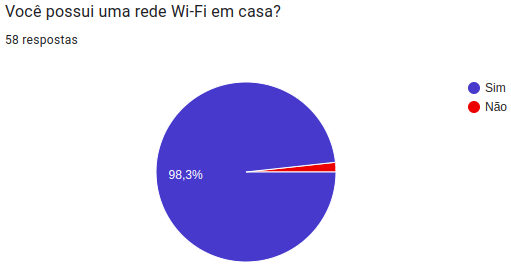
\includegraphics[width=.67\textwidth]{img/graf1-wifi.png}
    \caption{Uso de Wi-Fi dos alunos da EST. Fonte: Autor.}\label{figWifiAlunos}
\end{figure}

O último levantamento refere-se às expectativas em relação ao \textit{hardware}, destacando a preocupação com o uso do equipamento. Observou-se que apenas 37,9\% dos 
alunos já utilizaram algum dispositivo de automação residencial. Dessa forma, a solução proposta deve priorizar configurações simples, voltadas para usuários 
sem experiência prévia. 


\section{Especificação}\label{fase2}

A especificação é a etapa onde são definidas as funcionalidades do sistema embarcado e a modelagem da arquitetura e comunicação entre 
seus componentes. A partir das respostas, foram identificadas as principais funcionalidades 
para o sistema BURI, pois o desenvolvimento do sistema deve garantir que o protótipo final atenda às demandas reais do
público alvo. A funcionalidade de monitoramento em tempo real recebeu o maior número de votos (89,7\%) entre os participantes, porém opções como alerta de risco, fácil instalação e 
manutenção mínima foram requisitos proporcionalmente solicitados no questionário. 

\begin{figure}[ht]
    \centering
    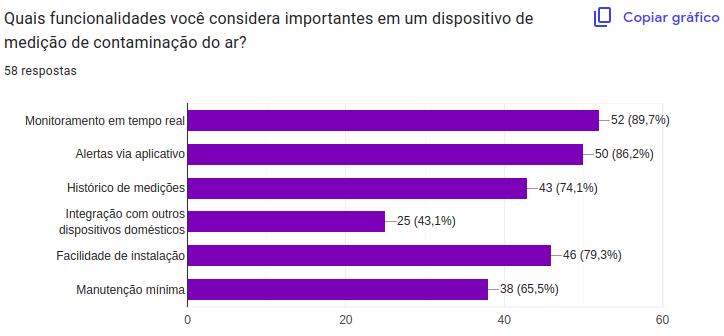
\includegraphics[width=.77\textwidth]{img/graf1-funcionalidades.png}
    \caption{Funcionalidades desejadas do sistema embarcado. Fonte: Autor.}\label{figFuncionalidades}
\end{figure}

Com base nas sugestões dos estudantes e considerando o prazo de entrega do trabalho de conclusão de curso, o escopo da proposta de solução contempla a 
implementação das seguintes funcionalidades: modo \textit{online} e \textit{offline}, monitoramento em tempo real, alerta de risco por notificação e processo de instalação facilitado.
As funcionalidades apresentadas têm o objetivo de equilibrar a expectativa dos usuários com a viabilidade técnica, pois a estrutura considera os recursos disponíveis e o prazo definido no 
cronograma.

O próximo passo da especificação é a modelagem de arquitetura do sistema, e para isso o projeto usa o padrão C4-model \cite{c4-model}. O C4 é um conjunto de ferramentas visuais usado pelo 
desenvolvedor de software na comunicação da arquitetura do sistema, semelhante a um mapa, com quatro níveis de detalhamento: \textit{context}, \textit{container}, \textit{component} e \textit{code}. A figura \ref{figContextDiagram} é o 
diagrama de contexto, por mostrar a comunicação via protocolo HTTP ou Blueetooth do usuário doméstico com a aplicação. A implementação do sistema tem como serviço externo a ferramenta Ngrok \cite{ngrok}, pois o uso do túnel HTTP e \textit{link} estático permite a API do \textit{backend} ser acessível tanto pelo equipamento 
embarcado quanto pelo aplicativo Android na internet.

\begin{figure}[ht]
    \centering
    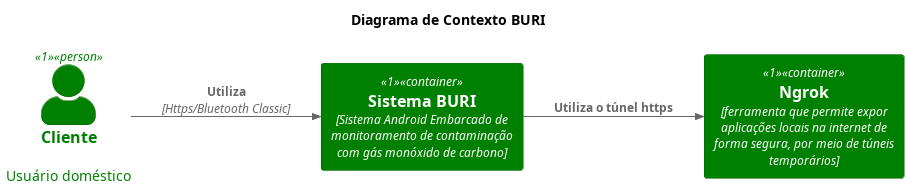
\includegraphics[width=.87\textwidth]{img/context-diagram.png}
    \caption{Diagrama de contexto. Fonte: Autor.}\label{figContextDiagram}
\end{figure}

O próximo diagrama é o de \textit{container}. Seu propósito é demonstrar o funcionamento da aplicação em termos de contêineres, ou seja, os elementos implantáveis
e componentes de software necessários para o pleno funcionamento do projeto. Na área de desenvolvimento de \textit{software}, o projeto possui três módulos principais: servidor, 
aplicativo e banco de dados. O servidor cuida das regras de negócio, como cadastro de usuários, dispositivos e login, mas também tem responsabilidade no 
armazenamento de medições do equipamento embarcado, cujo resultado é base para registro de eventos extremos. A segunda parte é o aplicativo Android. O módulo é a interface do sistema com o usuário doméstico, pois todo o fluxo de informação entre os 
diferentes componentes são fonte de dados para a visualização no \textit{smartphone} do indivíduo.

Por último, o Banco de Dados é responsável por armazenar todas as informações do sistema de monitoramento. Os dados de medição são organizados por dispositivo, onde 
cada um realiza o monitoramento de temperatura, umidade do ar e concentração de monóxido de carbono. Além disso, a estrutura de dados é otimizada para registrar tanto eventos críticos quanto 
medições dentro dos parâmetros normais.

\begin{figure}[ht]
    \centering
    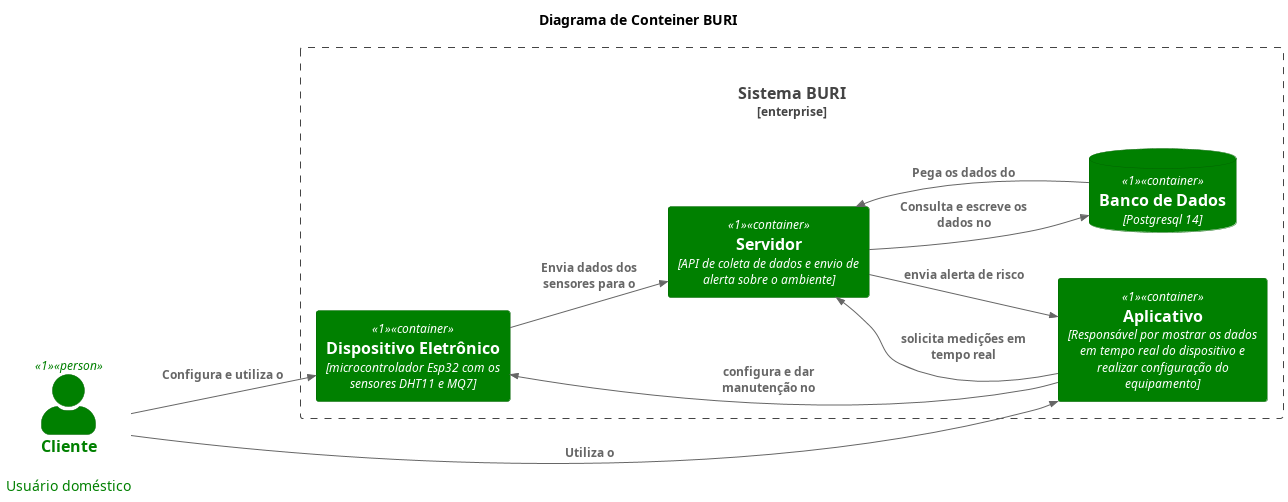
\includegraphics[width=.94\textwidth]{img/conteiner-diagram.png}
    \caption{Diagrama de container. Fonte: Autor.}\label{figConteinerDiagram}
\end{figure}

Sobre o \textit{hardware}, o sistema utiliza o dispositivo ESP32, juntamente com os sensores DHT11, para medição de temperatura e umidade do ar, e o MQ-7, para 
detecção de concentração de monóxido de carbono (CO). O microcontrolador atua no recebimento e envio de dados desses sensores e gerência da comunicação com o servidor ou aplicativo Android, mas seu funcionamento depende da energia da porta USB do 
notebook.

A próxima camada de abstração é o diagrama de componentes, no qual cada componente é responsável por um conjunto de tarefas bem definidas. Esses componentes interagem entre si por meio de interfaces ou contratos, 
garantindo a comunicação estruturada entre eles. A primeira representação é o diagrama de componentes do \textit{hardware}, pois ele detalha os sensores utilizados pelo microcontrolador, assim como 
os atuadores LED, usado na sinalização visual do modo de operação do circuito eletrônico, e o \textit{push button}, pois aciona a troca do modo de operação (\textit{online}/\textit{offline}) do dispositivo. Portanto, 
o \textit{hardware} também se comunica com o servidor e o aplicativo Android para envio de dados.

\begin{figure}[ht]
    \centering
    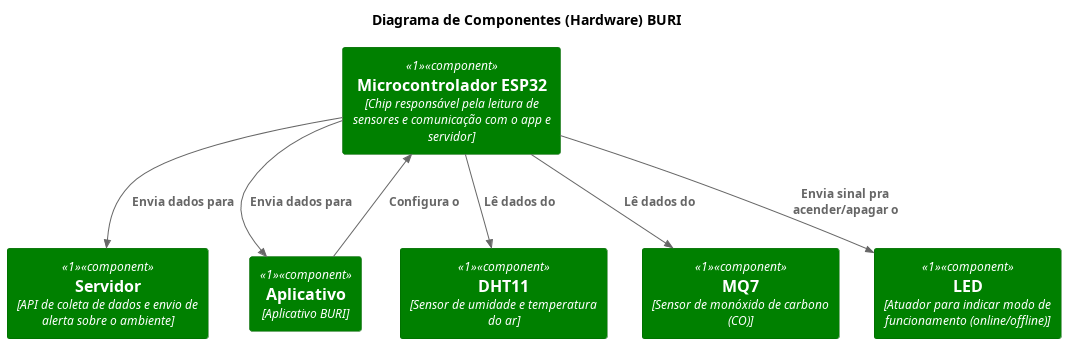
\includegraphics[width=.88\textwidth]{img/component-diagram-hardware.png}
    \caption{Diagrama de Componente (\textit{Hardware}). Fonte: Autor.}\label{figComponentHardware}
\end{figure}

Por último, será apresentado o diagrama de componentes do \textit{software}. O servidor tem acesso direto ao banco de dados e possui três principais controladores: \textit{Account Controller}, \textit{Measurement Controller} e \textit{Event Controller}. 

O primeiro gerencia os dados de usuário e seus dispositivos cadastrados, além de configurar o processo de autenticação e \textit{login} via dados de email e senha. Em seguida, o \textit{Measurement Controller} é interface de recebimento dos dados de cada dispositivo eletrônico, assim como 
o compartilhamento de informação com o aplicativo Android. O \textit{Event Controller} é o principal responsável na emissão de alerta de risco no aplicativo, pois o controlador recebe os dados em tempo real do banco de dados e avalia, 
com base em alguns parâmetros, se o ambiente possui comportamento perigoso, gerando o registro de um novo evento no banco de dados.

\begin{figure}[ht]
    \centering
    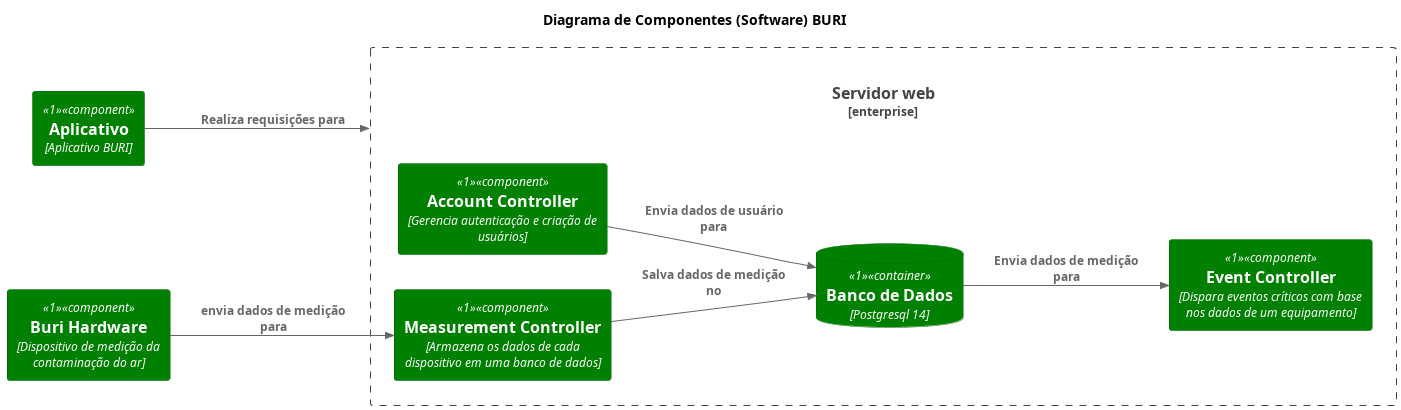
\includegraphics[width=.94\textwidth]{img/component-diagram-software.png}
    \caption{Diagrama de Componente (\textit{Software}). Fonte: Autor.}\label{figComponentSoftware}
\end{figure}

\section{Particionamento (Hw/Sw)}\label{fase3}

Após a conclusão da especificação, inicia-se o particionamento das atividades. Esse processo envolve a divisão do trabalho em tarefas menores, facilitando 
a organização, a alocação de recursos e a mensuração do progresso durante a fase de desenvolvimento. Portanto, as atividades de \textit{software} (Sw) são definidas de acordo 
com a lista a seguir.

\begin{itemize}
    \item Desenvolvimento da modelagem e implantação do Banco de Dados;
    \item Implementação da API:
    \begin{itemize}
        \item Rota de gerenciamento de conta de usuário;
        \item Rota de Medição em tempo real por dispositivo;
        \item Rota de Eventos do ambiente;
    \end{itemize}
    \item Desenvolvimento do Aplicativo Android;
    \item Codificação do \textit{firmware} no ESP32;
\end{itemize}

Além das atividades de \textit{software}, o particionamento abrange também as atividades relacionadas ao \textit{hardware} (Hw). Essas atividades focam na concepção, desenvolvimento e montagem dos componentes 
eletrônicos do sistema, garantindo os requisitos definidos na especificação. As atividades de \textit{hardware} são descritas a seguir:

\begin{itemize}
    \item Escolha e estudo dos componentes eletrônicos;
    \item Implementação do controle do LED por botão;
    \item Montagem do circuito e verificação de leitura dos sensores;
    \item Configuração dos modos \textit{online} e \textit{offline};
\end{itemize}

A construção da proposta é o resultado da junção entre as duas áreas. Porém, desenvolver o sistema embarcado 
na metodologia iterativo e incremental exige o conhecimento prévio da dependência de serviços entre as partes, assim como o uso de protocolos 
de comunicação do início ao fim do projeto. Dito isso, a figura \ref{figTarefasMetodologia} ilustra a organização das tarefas de HW e SW, considerando 
a integração entre os componentes logicamente dependentes dentro de cada iteração.

\begin{figure}[ht]
    \centering
    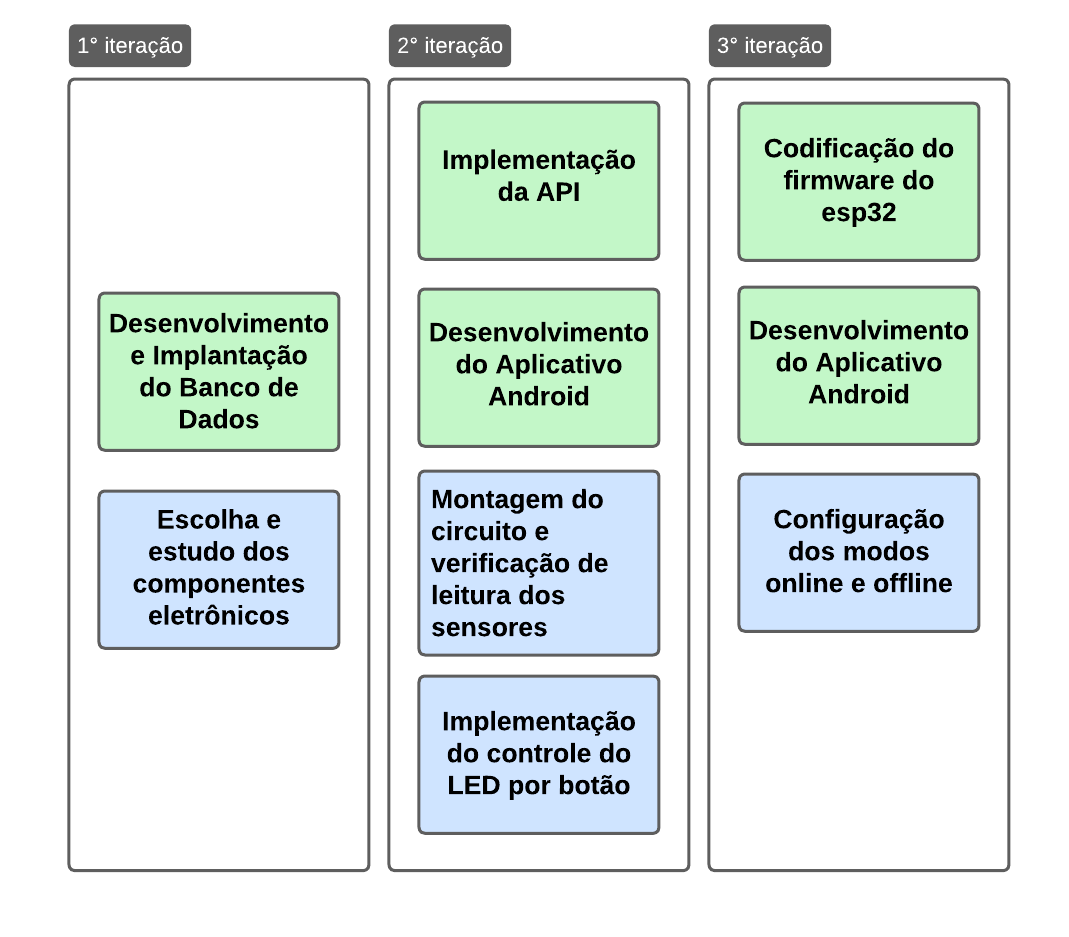
\includegraphics[width=.44\textwidth]{img/tarefas-metodologia.png}
    \caption{Organização de tarefas. Fonte: Autor.}\label{figTarefasMetodologia}
\end{figure}

\section{Execução de Atividades}\label{fase4}

Esta seção tem em vista detalhar os procedimentos adotados para a execução das atividades estabelecidas na etapa anterior. O desenvolvimento 
integrado de \textit{hardware} e \textit{software} exige uma abordagem iterativa, na qual funcionalidades específicas de uma área são projetadas para interagir com 
a outra, garantindo o sucesso na implementação do sistema.

\subsection{Primeira iteração}\label{ExecAtv1It}

A primeira atividade de \textit{software} diz respeito ao Banco de Dados, pois as informações de toda a aplicação 
precisam de registro e persistência. ``Um banco de dados representa algum aspecto do mundo real, às vezes chamado de minimundo ou de universo de discurso'' \cite[pp. 3]{banco-de-dados-navathe2014}. Assim como na engenharia de \textit{software}, o projeto 
de um banco de dados surge na análise de requisitos, pois nela são definidas as restrições e propriedades de cada conceito do mundo real cuja abstração 
deve ser persistida para futuras consultas. Portanto, o sistema BURI utiliza o Banco de Dados relacional \textit{PostgreSQL} e implementa a construção de tabelas 
via ORM (do inglês, \textit{Object Relational Mapper}), pois é uma técnica que permite o mapeamento dos objetos com os dados armazenados no sistema de banco de dados \cite{hibernate-documentation}. 

\begin{figure}[ht]
    \centering
    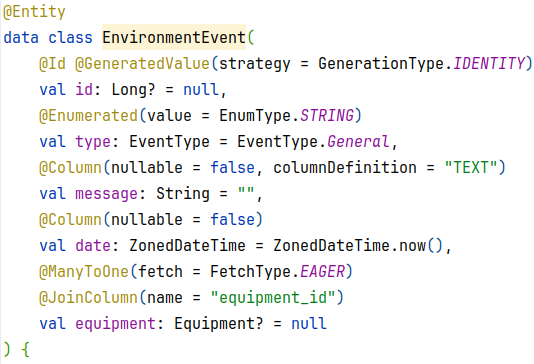
\includegraphics[width=0.45\textwidth]{img/event-class-kotlin.png}
    \hfill
    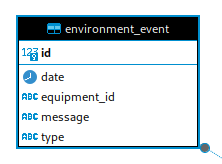
\includegraphics[width=0.42\textwidth]{img/event-table-postgres.png}
    \caption{Mapeamento Objeto Relacional da classe Evento. Fonte: Autor.}\label{figJpaEvent}
\end{figure}

Por outro lado, o \textit{Java Persistence API}, também conhecido pela sigla JPA, é uma camada 
de abstração do \textit{framework} para persistência de dados \cite{spring-data-jpa-documentation}. Seu papel 
é simplificar a operação com banco de dados relacionais, pois os desenvolvedores de \textit{software} utilizam objetos Java 
em vez de instruções SQL diretamente. Além disso, o projeto define um padrão de mapeamento de objetos para tabelas com base em anotações e
oferece recursos avançados de consulta via implementações do padrão de projeto \textit{Repository}. O esquema de Banco de Dados resultou na criação das 
tabelas e relacionamentos ilustrados na figura \ref{figSchemaBuriDB}.

\begin{figure}[ht]
    \centering
    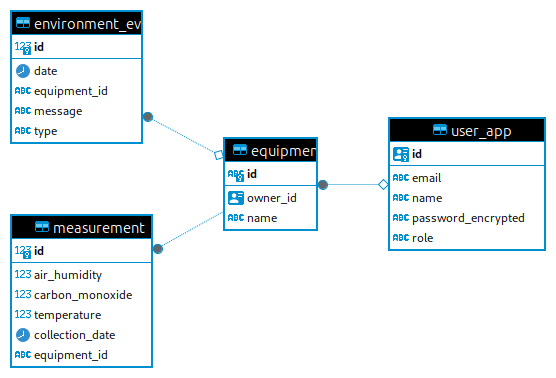
\includegraphics[width=.54\textwidth]{img/buri_schema_bd.png}
    \caption{Esquema do Banco de Dados BURI. Fonte: Autor.}\label{figSchemaBuriDB}
\end{figure}

No modelo, o usuário pode obter vários dispositivos e cada dispositivo tem a responsabilidade de atualizar as tabelas de medição e evento 
a partir da conexão por Wi-Fi com o servidor. Porém, o servidor possui uma rotina de verificação da medição atual antes de inserir no banco de dados 
para o sistema poder identificar se os valores registrados correspondem a um evento crítico ou não. 

A atividade de \textit{hardware} desta etapa consiste na pesquisa e estudo dos componentes eletrônicos. Conforme as variáveis de interesse deste trabalho de 
conclusão de curso, os sensores de medição escolhidos foram o DHT11 e o MQ-7, os mesmos utilizados no trabalho acadêmico \textit{AirWorld} \cite{UFAMAirWorld}. Uma vez definido os sensores, 
o próximo passo consiste na escolha do microcontrolador, pois ele será responsável por gerenciar as leituras dos sensores, processar os dados e comunicar-se com o servidor para armazenar as medições.

O ESP32 foi escolhido devido à sua versatilidade, ao possuir conectividade Wi-Fi e Bluetooth integradas, o que facilita a comunicação sem fio com outros componentes do sistema de monitoramento. Além disso, destaca-se 
pela robustez e poder de processamento, ao oferecer maior velocidade de processamento em comparação com outras opções, o que é essencial para o desempenho do sistema. Outro destaque é a economia, já que o microcontrolador 
é relativamente acessível, quando comparado a outras placas de desenvolvimento com funcionalidades semelhantes, tornando-o ideal para o desenvolvimento rápido de aplicações, pois a análise da figura \ref{figTableEsp} fundamenta a decisão.

Em seguida, foi realizada a aquisição dos materiais necessários para o desenvolvimento do projeto, incluindo os sensores, o microcontrolador e outros componentes eletrônicos essenciais para a implementação do circuito. A compra dos itens 
otimizou os recursos financeiros e atendeu às especificações técnicas do projeto embarcado. Para tanto, são apresentados a seguir os custos da solução proposta na tabela \ref{tabPrecoHardware}.

\begin{table}[h!]
    \centering
    \begin{tabular}{|c|c|c|}
        \hline
        \textbf{Quantidade} & \textbf{Nome do componente} & \textbf{Custo R\$} \\
        \hline
        1 & DHT11 - Sensor de umidade e temperatura & 15,50 \\
        \hline
        1 & MQ-7 - Sensor de monóxido de carbono & 32,00 \\
        \hline
        1 & WROOM-32 ESP32S - 30 Pinos & 58,00 \\
        \hline
        1 & Resistor 30 Ohms 5\% & 0,20 \\
        \hline
        1 & Resistor 200 kOhms 5\% & 0,40 \\
        \hline
        1 & LED difuso verde 5mm & 0,40 \\
        \hline
        1 & Botão \textit{push button} chave táctil & 0,25 \\
        \hline
        10 & 1 Kit Jumper Macho-Fêmea & 5,00 \\
        \hline
        10 & 1 Kit Jumper Fêmea-Fêmea & 5,00 \\
        \hline
        10 & 1 Kit Jumper Macho-Macho & 5,00 \\
        \hline
        1 & Cabo de Dados USB V8 Micro USB & 9,50 \\
        \hline
        1 & Protoboard 400 furos & 15,00 \\
        \hline
        \textbf{--} & \textbf{Custo Total} & \textbf{146,25} \\
        \hline
    \end{tabular}
    \caption{Custo total de componentes eletrônicos para a prototipação do \textit{hardware}. Os preços são de lojas em Manaus no período de abril a julho de 2024. Fonte: Autor.}\label{tabPrecoHardware}
\end{table}

%O DHT11 é um sensor de leitura digital comumente utilizado em projetos de automação para medir temperatura e umidade do ar. O dispositivo possui um rigoroso processo de calibração, assim como 
%tamanho reduzido e baixo consumo de energia. Composto por quatro pinos: VCC, responsável pela alimentação do sensor (3.3V ou 5V); GND, que conecta ao sinal terra do circuito; DATA, responsável pela trasmissão 
%de dados digitais; e NC, um pino sem utilidade.

\subsection{Segunda iteração}\label{ExecAtv2It}

\subsection{Terceira iteração}\label{ExecAtv3It}

\section{Testes de aceitação}\label{fase5}

\section{Documentação}\label{fase6}